\chapterimage{chapter_head_1.pdf}
\chapter{Strings}
\label{strings}


\section{A string is a sequence}
\index{sequence}
\index{character}
\index{bracket operator}
\index{operator!bracket}

A string is a {\bf sequence} of characters.  
You can access the characters one at a time with the
bracket operator:

\beforeverb
\begin{pyinterpreter}
>>> fruit = 'banana'
>>> letter = fruit[1]
\end{pyinterpreter}
\afterverb
%
The second statement selects character number 1 from {\tt
fruit} and assigns it to {\tt letter}.  
%
\index{index}
%
The expression in brackets is called an {\bf index}.  
The index indicates which character in the sequence you
want (hence the name).
%
But you might not get what you expect:

\beforeverb
\begin{pyinterpreter}
>>> print(letter)
a
\end{pyinterpreter}
\afterverb
%
For most people, the first letter of \verb"'banana'" is {\tt b}, not
{\tt a}.  But for computer scientists, the index is an offset from the
beginning of the string, and the offset of the first letter is zero.

\beforeverb
\begin{pyinterpreter}
>>> letter = fruit[0]
>>> print(letter)
b
\end{pyinterpreter}
\afterverb
%
So {\tt b} is the 0th letter (``zero-eth'') of \verb"'banana'", {\tt a}
is the 1th letter (``one-eth''), and {\tt n} is the 2th (``two-eth'')
letter.

\index{index!starting at zero}
\index{zero, index starting at}

You can use any expression, including variables and operators, as an
index, but the value of the index has to be an integer.  Otherwise you
get:

\index{index}
\index{exception!TypeError}
\index{TypeError}

\beforeverb
\begin{pyinterpreter}
>>> letter = fruit[1.5]
TypeError: string indices must be integers
\end{pyinterpreter}
\afterverb
%

\section{Function {\tt len}}

\index{len function}
\index{function!len}

{\tt len} is a built-in function that returns the number of characters
in a string:

\beforeverb
\begin{pyinterpreter}
>>> fruit = 'banana'
>>> len(fruit)
6
\end{pyinterpreter}
\afterverb
%
To get the last letter of a string, you might be tempted to try something
like this:

\index{exception!IndexError}
\index{IndexError}

\beforeverb
\begin{pyinterpreter}
>>> length = len(fruit)
>>> last = fruit[length]
IndexError: string index out of range
\end{pyinterpreter}
\afterverb
%
The reason for the {\tt IndexError} is that there is no letter in {\tt
'banana'} with the index 6.  Since we started counting at zero, the
six letters are numbered 0 to 5.  To get the last character, you have
to subtract 1 from {\tt length}:

\beforeverb
\begin{pyinterpreter}
>>> last = fruit[length-1]
>>> print(last)
a
\end{pyinterpreter}
\afterverb
%
Alternatively, you can use negative indices, which count backward from
the end of the string.  The expression {\tt fruit[-1]} yields the last
letter, {\tt fruit[-2]} yields the second to last, and so on.

\index{index!negative}
\index{negative index}


\section{Traversal with a {\tt for} loop}
\label{for}

\index{traversal}
\index{loop!traversal}
\index{for loop}
\index{loop!for}
\index{statement!for}
\index{traversal}

A lot of computations involve processing a string one character at a
time.  Often they start at the beginning, select each character in
turn, do something to it, and continue until the end.  This pattern of
processing is called a {\bf traversal}.  One way to write a traversal
is with a {\tt while} loop:

\beforeverb
\begin{pycode}
index = 0
while index < len(fruit):
    letter = fruit[index]
    print(letter)
    index = index + 1
\end{pycode}
\afterverb
%
This loop traverses the string and displays each letter on a line by
itself.  The loop condition is {\pyinline/index < len(fruit)/}, so
when {\tt index} is equal to the length of the string, the
condition is false, and the body of the loop is not executed.  The
last character accessed is the one with the index {\tt len(fruit)-1},
which is the last character in the string.

\begin{exercise}
Write a function that takes a string as an argument
and displays the letters backward, one per line.
\end{exercise}

Another way to write a traversal is with a {\tt for} loop:

\beforeverb
\begin{pycode}
for char in fruit:
    print(char)
\end{pycode}
\afterverb
%
Each time through the loop, the next character in the string is assigned
to the variable {\tt char}.  The loop continues until no characters are
left.

\index{concatenation}
\index{abecedarian}
\index{McCloskey, Robert}

The following example shows how to use concatenation (string addition)
and a {\tt for} loop to generate an abecedarian series (that is, in
alphabetical order).  In Robert McCloskey's book {\em Make
Way for Ducklings}, the names of the ducklings are Jack, Kack, Lack,
Mack, Nack, Ouack, Pack, and Quack.  This loop outputs these names in
order:

\beforeverb
\begin{pycode}
prefixes = 'JKLMNOPQ'
suffix = 'ack'

for letter in prefixes:
    print(letter + suffix)
\end{pycode}
\afterverb
%
The output is:

\beforeverb
\begin{pyoutput}
Jack
Kack
Lack
Mack
Nack
Oack
Pack
Qack
\end{pyoutput}
\afterverb
%
Of course, that's not quite right because ``Ouack'' and
``Quack'' are misspelled.

\begin{exercise}
Modify the program to fix this error.
\end{exercise}



\section{String slices}
\label{slice}

\index{slice operator}
\index{operator!slice}
\index{index!slice}
\index{string!slice}
\index{slice!string}

A segment of a string is called a {\bf slice}.  Selecting a slice is
similar to selecting a character:

\beforeverb
\begin{pyinterpreter}
>>> s = 'Monty Python'
>>> print(s[0:5])
Monty
>>> print(s[6:12])
Python
\end{pyinterpreter}
\afterverb
%
The operator {\pyinline/[n:m]/} returns the part of the string from the 
``n-eth'' character to the ``m-eth'' character, including the first but
excluding the last.  This behavior is counter intuitive, but it might
help to imagine the indices pointing {\em between} the
characters, as in the following diagram:

\beforefig
\centerline{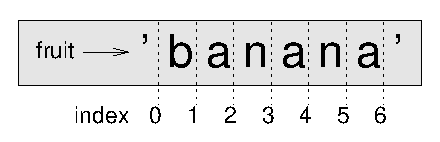
\includegraphics{figs/banana.eps}}
\afterfig

If you omit the first index (before the colon), the slice starts at
the beginning of the string.  If you omit the second index, the slice
goes to the end of the string:

\beforeverb
\begin{pyinterpreter}
>>> fruit = 'banana'
>>> fruit[:2]
'bana'
>>> fruit[2:]
'nana'
\end{pyinterpreter}
\afterverb
%
If the first index is greater than or equal to the second the result
is an {\bf empty string}, represented by two quotation marks:

\index{quotation mark}

\beforeverb
\begin{pyinterpreter}
>>> fruit = 'banana'
>>> fruit[3:3]
''
\end{pyinterpreter}
\afterverb
%
An empty string contains no characters and has length 0, but other
than that, it is the same as any other string.

\begin{exercise}
Given that {\tt fruit} is a string, what does
{\tt fruit[:]} mean?

\index{copy!slice}
\index{slice!copy}


\end{exercise}


\section{Strings are immutable}
\index{mutability}
\index{immutability}
\index{string!immutable}

It is tempting to use the {\tt [ ]} operator on the left side of an
assignment, with the intention of changing a character in a string.
For example:

\index{TypeError}
\index{exception!TypeError}

\beforeverb
\begin{pyinterpreter}
>>> greeting = 'Hello, world!'
>>> greeting[0] = 'J'
TypeError: object does not support item assignment
\end{pyinterpreter}
\afterverb
%
The ``object'' in this case is the string and the ``item'' is
the character you tried to assign.  For now, an {\bf object} is
the same thing as a value, but we will refine that definition
later.  An {\bf item} is one of the values in a sequence.
%
\index{object}
\index{item assignment}
\index{assignment!item}
\index{immutability}
%
The reason for the error is that
strings are {\bf immutable}, which means you can't change an
existing string.  The best you can do is create a new string
that is a variation on the original:

\beforeverb
\begin{pyinterpreter}
>>> greeting = 'Hello, world!'
>>> new_greeting = 'J' + greeting[1:]
>>> print(new_greeting)
Jello, world!
\end{pyinterpreter}
\afterverb
%
This example concatenates a new first letter onto
a slice of {\tt greeting}.  It has no effect on
the original string.

\index{concatenation}


\section{Searching}
\label{find}

What does the following function do?

\index{find function}
\index{function!find}

\beforeverb
\begin{pycode}
def find(word, letter):
    index = 0
    while index < len(word):
        if word[index] == letter:
            return index
        index = index + 1
    return -1
\end{pycode}
\afterverb
%
In a sense, {\tt find} is the opposite of the {\tt [ ]} operator.
Instead of taking an index and extracting the corresponding character,
it takes a character and finds the index where that character
appears.  If the character is not found, the function returns {\tt
-1}.
%
This is the first example we have seen of a {\tt return} statement
inside a loop.  If {\tt word[index] == letter}, the function breaks
out of the loop and returns immediately.
%
If the character doesn't appear in the string, the program
exits the loop normally and  returns {\tt -1}.
%
This pattern of computation---traversing a sequence and returning
when we find what we are looking for---is called a {\bf search}.

\index{traversal}
\index{search pattern}
\index{pattern!search}

\begin{exercise}
Modify {\tt find} so that it has a
third parameter, the index in {\tt word} where it should start
looking.
\end{exercise}


\section{Looping and counting}
\label{counter}

\index{counter}
\index{counting and looping}
\index{looping and counting}
\index{looping!with strings}

The following program counts the number of times the letter {\tt a}
appears in a string:

\beforeverb
\begin{pycode}
word = 'banana'
count = 0
for letter in word:
    if letter == 'a':
        count = count + 1
print(count)
\end{pycode}
\afterverb
%
This program demonstrates another pattern of computation called a {\bf
counter}.  The variable {\tt count} is initialized to 0 and then
incremented each time an {\tt a} is found.
When the loop exits, {\tt count}
contains the result---the total number of {\tt a}'s.

\begin{exercise}
\index{encapsulation}

Encapsulate this code in a function named {\tt
count}, and generalize it so that it accepts the string and the
letter as arguments.
\end{exercise}

\begin{exercise}
Rewrite this function so that instead of
traversing the string, it uses the three-parameter version of {\tt
find} from the previous section.
\end{exercise}


\section{{\tt string} methods}

A {\bf method} is similar to a function---it takes arguments and
may return a value---but the syntax is different.  For example, the
method {\tt upper} takes a string and returns a new string with
all uppercase letters:
%
\index{method}
\index{string!method}
%
Instead of the function syntax {\tt upper(word)}, it uses
the method syntax {\tt word.upper()}.

\index{dot notation}

\beforeverb
\begin{pyinterpreter}
>>> word = 'banana'
>>> new_word = word.upper()
>>> print(new_word)
BANANA
\end{pyinterpreter}
\afterverb
%
This form of dot notation specifies the name of the method, {\tt
upper}, and the name of the string to apply the method to, {\tt
word}.  The empty parentheses indicate that this method takes no
argument.

\index{parentheses!empty}

A method call is called an {\bf invocation}; in this case, we would
say that we are invoking {\tt upper} on the {\tt word}.
%
\index{invocation}
%
As it turns out, there is a string method named {\tt find} that
is remarkably similar to the function we wrote:

\beforeverb
\begin{pyinterpreter}
>>> word = 'banana'
>>> index = word.find('a')
>>> print(index)
1
\end{pyinterpreter}
\afterverb
%
In this example, we invoke {\tt find} on {\tt word} and pass
the letter we are looking for as a parameter.
%
Actually, the {\tt find} method is more general than our function;
it can find substrings, not just characters:

\beforeverb
\begin{pyinterpreter}
>>> word.find('na')
2
\end{pyinterpreter}
\afterverb
%
It can take as a second argument the index where it should start:

\index{optional argument}
\index{argument!optional}

\beforeverb
\begin{pyinterpreter}
>>> word.find('na', 3)
4
\end{pyinterpreter}
\afterverb
%
And as a third argument the index where it should stop:

\beforeverb
\begin{pyinterpreter}
>>> name = 'bob'
>>> name.find('b', 1, 2)
-1
\end{pyinterpreter}
\afterverb
%
This search fails because {\tt b} does not
appear in the index range from {\tt 1} to {\tt 2} (not including {\tt
2}).


\begin{exercise}
\index{count method}
\index{method!count}

There is a string method called {\tt count} that is similar
to the function in the previous exercise.  Read the documentation
of this method
and write an invocation that counts the number of {\tt a}
in \verb"'banana'".
\end{exercise}


\section{The {\tt in} operator}
\label{inboth}

\index{in operator}
\index{operator!in}
\index{boolean operator}
\index{operator!boolean}

The word {\tt in} is a boolean operator that takes two strings and
returns {\tt True} if the first appears as a substring in the second:

\beforeverb
\begin{pyinterpreter}
>>> 'ana' in 'banana'
True
>>> 'rama' in 'banana'
False
\end{pyinterpreter}
\afterverb
%
For example, the following function prints all the
letters from {\tt word1} that also appear in {\tt word2}:

\beforeverb
\begin{pycode}
def in_both(word1, word2):
    for letter in word1:
        if letter in word2:
            print(letter)
\end{pycode}
\afterverb
%
With well-chosen variable names,
Python sometimes reads like English.  You could read
this loop, ``for (each) letter in (the first) word, if (the) letter 
(appears) in (the second) word, print (the) letter.''

Here's what you get if you compare apples and oranges:

\beforeverb
\begin{pyinterpreter}
>>> in_both('apples', 'oranges')
a
e
s
\end{pyinterpreter}
\afterverb
%

\section{String comparison}

\index{string!comparison}
\index{comparison!string}

The relational operators work on strings.  To see if two strings are equal:

\beforeverb
\begin{pycode}
if word == 'banana':
    print ('All right, bananas.')
\end{pycode}
\afterverb
%
Other relational operations are useful for putting words in alphabetical
order:

\beforeverb
\begin{pycode}
if word < 'banana':
    print('Your word,' + word + ', comes before banana.')
elif word > 'banana':
    print('Your word,' + word + ', comes after banana.')
else:
    print('All right, bananas.')
\end{pycode}
\afterverb
%
%Python does not handle uppercase and lowercase letters the same way
%that people do.  All the uppercase letters come before all the
%lowercase letters, so:
%
%\beforeverb
%\begin{pycode}
%Your word, Pineapple, comes before banana.
%\end{pycode}
%\afterverb
%%
%A common way to address this problem is to convert strings to a
%standard format, such as all lowercase, before performing the
%comparison.  Keep that in mind in case you have to defend yourself
%against a man armed with a Pineapple.


\section{Debugging}
\index{debugging}

\index{traversal}

When you use indices to traverse the values in a sequence,
it is tricky to get the beginning and end of the traversal
right.  Here is a function that is supposed to compare two
words and return {\tt True} if one of the words is the reverse
of the other, but it contains two errors:

\beforeverb
\begin{pycode}
def is_reverse(word1, word2):
    if len(word1) != len(word2):
        return False
    
    i = 0
    j = len(word2)

    while j > 0:
        if word1[i] != word2[j]:
            return False
        i = i+1
        j = j-1

    return True
\end{pycode}
\afterverb
%
The first {\tt if} statement checks whether the words are the
same length.  If not, we can return {\tt False} immediately
and then, for the rest of the function, we can assume that the words
are the same length.  This is an example of the guardian pattern
in Section~\ref{guardian}.
%
\index{guardian pattern}
\index{pattern!guardian}
\index{index}
%
{\tt i} and {\tt j} are indices: {\tt i} traverses {\tt word1}
forward while {\tt j} traverses {\tt word2} backward.  If we find
two letters that don't match, we can return {\tt False} immediately.
If we get through the whole loop and all the letters match, we
return {\tt True}.

If we test this function with the words ``pots'' and ``stop'', we
expect the return value {\tt True}, but we get an IndexError:

\index{IndexError}
\index{exception!IndexError}

\beforeverb
\begin{pyinterpreter}
>>> is_reverse('pots', 'stop')
...
  File "reverse.py", line 15, in is_reverse
    if word1[i] != word2[j]:
IndexError: string index out of range
\end{pyinterpreter}
\afterverb
%
For debugging this kind of error, my first move is to
print the values of the indices immediately before the line
where the error appears.

\beforeverb
\begin{pycode}
    while j > 0:
        print(i, j)        # print here
        
        if word1[i] != word2[j]:
            return False
        i = i+1
        j = j-1
\end{pycode}
\afterverb
%
Now when I run the program again, I get more information:

\beforeverb
\begin{pyinterpreter}
>>> is_reverse('pots', 'stop')
0 4
...
IndexError: string index out of range
\end{pyinterpreter}
\afterverb
%
The first time through the loop, the value of {\tt j} is 4,
which is out of range for the string \verb"'pots'".
The index of the last character is 3, so the
initial value for {\tt j} should be {\tt len(word2)-1}.

\index{semantic error}
\index{error!semantic}

If I fix that error and run the program again, I get:

\beforeverb
\begin{pyinterpreter}
>>> is_reverse('pots', 'stop')
0 3
1 2
2 1
True
\end{pyinterpreter}
\afterverb
%
This time we get the right answer, but it looks like the loop only ran
three times, which is suspicious.  To get a better idea of what is
happening, it is useful to draw a state diagram.  During the first
iteration, the frame for \verb"is_reverse" looks like this:

\index{state diagram}
\index{diagram!state}

\beforefig
\centerline{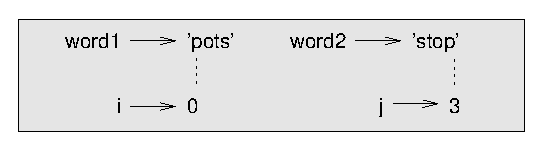
\includegraphics{figs/state4.eps}}
\afterfig

I took a little license by arranging the variables in the frame
and adding dotted lines to show that the values of {\tt i} and
{\tt j} indicate characters in {\tt word1} and {\tt word2}.

\begin{exercise}
\label{is_reverse}
Starting with this diagram, execute the program on paper, changing the
values of {\tt i} and {\tt j} during each iteration.  Find and fix the
second error in this function.
\end{exercise}



\section{Glossary}
	
\begin{vocabulary}[object:] Something a variable can refer to.  For now,
you can use ``object'' and ``value'' interchangeably.
\index{object}
\end{vocabulary}
	
\begin{vocabulary}[sequence:] An ordered set; that is, a set of
values where each value is identified by an integer index.
\index{sequence}
\end{vocabulary}
	
\begin{vocabulary}[item:] One of the values in a sequence.
\index{item}
\end{vocabulary}
	
\begin{vocabulary}[index:] An integer value used to select an item in
a sequence, such as a character in a string.
\index{index}
\end{vocabulary}
	
\begin{vocabulary}[slice:] A part of a string specified by a range of indices.
\index{slice}
\end{vocabulary}
	
\begin{vocabulary}[empty string:] A string with no characters and length 0, represented
by two quotation marks.
\index{empty string}
\end{vocabulary}
	
\begin{vocabulary}[immutable:] The property of a sequence whose items cannot
be assigned.
\index{immutability}
\end{vocabulary}
	
\begin{vocabulary}[traverse:] To iterate through the items in a sequence,
performing a similar operation on each.
\index{traversal}
\end{vocabulary}
	
\begin{vocabulary}[search:] A pattern of traversal that stops
when it finds what it is looking for.
\index{search pattern}
\index{pattern!search}
\end{vocabulary}
	
\begin{vocabulary}[counter:] A variable used to count something, usually initialized
to zero and then incremented.
\index{counter}
\end{vocabulary}
	
\begin{vocabulary}[method:] A function that is associated with an object and called
using dot notation.
\index{method}
\end{vocabulary}
	
\begin{vocabulary}[invocation:] A statement that calls a method.
\index{invocation}
\end{vocabulary}
	


\section{Exercises}

\begin{exercise}

\index{step size}
\index{slice operator}
\index{operator!slice}

A string slice can take a third index that specifies the ``step
size;'' that is, the number of spaces between successive characters.
A step size of 2 means every other character; 3 means every third,
etc.

\beforeverb
\begin{pyexo}
>>> fruit = 'banana'
>>> fruit[0:5:2]
'bnn'
\end{pyexo}
\afterverb

A step size of -1 goes through the word backwards, so
the slice \verb"[::-1]" generates a reversed string.
%
\index{palindrome}
%
Use this idiom to write a one-line version of \verb"is_palindrome"
from Exercise~\ref{palindrome}.
\end{exercise}


\begin{exercise}
\index{string method}
\index{method!string}

Read the documentation of the string methods at
\url{docs.python.org/lib/string-methods.html}.  You
might want to experiment with some of them to make sure
you understand how they work.  {\tt strip} and
{\tt replace} are particularly useful.
%
The documentation uses a syntax that might be confusing.
For example, in \verb"find(sub[, start[, end]])", the brackets
indicate optional arguments.  So {\tt sub} is required, but
{\tt start} is optional, and if you include {\tt start},
then {\tt end} is optional.
\end{exercise}

\begin{exercise}
The following functions are all {\em intended} to check whether a
string contains any lowercase letters, but at least some of them are
wrong.  For each function, describe what the function actually does
(assuming that the parameter is a string).

\begin{pyexo}
def any_lowercase1(s):
    for c in s:
        if c.islower():
            return True
        else:
            return False
\end{pyexo}

\begin{pyexo}
def any_lowercase2(s):
    for c in s:
        if 'c'.islower():
            return 'True'
        else:
            return 'False'
\end{pyexo}

\begin{pyexo}
def any_lowercase3(s):
    for c in s:
        flag = c.islower()
    return flag
\end{pyexo}

\begin{pyexo}
def any_lowercase4(s):
    flag = False
    for c in s:
        flag = flag or c.islower()
    return flag
\end{pyexo}

\begin{pyexo}
def any_lowercase5(s):
    for c in s:
        if not c.islower():
            return False
    return True
\end{pyexo}

\end{exercise}


\begin{exercise}
\index{letter rotation}
\index{rotation, letter}

\label{exrotate}
ROT13 is a weak form of encryption that involves ``rotating'' each
letter in a word by 13 places\footnote{See
  \url{wikipedia.org/wiki/ROT13}.}.  To rotate a letter means
to shift it through the alphabet, wrapping around to the beginning if
necessary, so 'A' shifted by 3 is 'D' and 'Z' shifted by 1 is 'A'.

Write a function called \verb"rotate_word"
that takes a string and an integer as parameters, and that returns
a new string that contains the letters from the original string
``rotated'' by the given amount.  

For example, ``cheer'' rotated by 7 is ``jolly'' and ``melon'' rotated
by -10 is ``cubed''.  
%
%%For example ``sleep''
%%rotated by 9 is ``bunny'' and ``latex'' rotated by 7 is ``shale''.
%
You might want to use the built-in functions {\tt ord}, which converts
a character to a numeric code, and {\tt chr}, which converts numeric
codes to characters.
%
%Potentially offensive jokes on the Internet are sometimes encoded
%in ROT13.  If you are not easily offended, find and decode some
%of them.
\end{exercise}
